\chapter{Experimental Models}
\hspace{0.5cm} In this chapter, we are going to propose two architecture alterations to the DeepSORT\cite{Wojke2017simple} in order to
improve performance of DeepSORT\cite{Wojke2017simple} in MOT16-train dataset\cite{Milan2016MOT16AB}.
\section{DeepSORT with Parameter-free Spatial Attention to extract deep appearance features}
\hspace{0.5cm} One of the most difficult problem to handle in pedestrian tracking is re-identification. Re-identification problem comes from the limitation of
FOV\footnote{Field Of View} of camera, partially or fully occlusion and
reappearance . In the DeepSORT \cite{Wojke2017simple}, authors proposed an
appearance metric that uses feature vectors extracted from a CNN to compare to
gallery of features of successfuly tracked objects from 100 previous
frames in order to identify current target. However, the CNN architecture is
over simply and do not archive competitive result on these
re-identification datasets, theoretically, replacing mentioned CNN
architecture by a stronger or better model in person re-identification
challenge would provide a more accurate measurement to re-identify pedestrian.\par
The \cite{SA} currently provides state-of-the-art results which is shown in fig.\ref{fig:sa_results} on almost large-scale person
re-identification dataset.\par
\begin{figure}[h!]
    \centering
    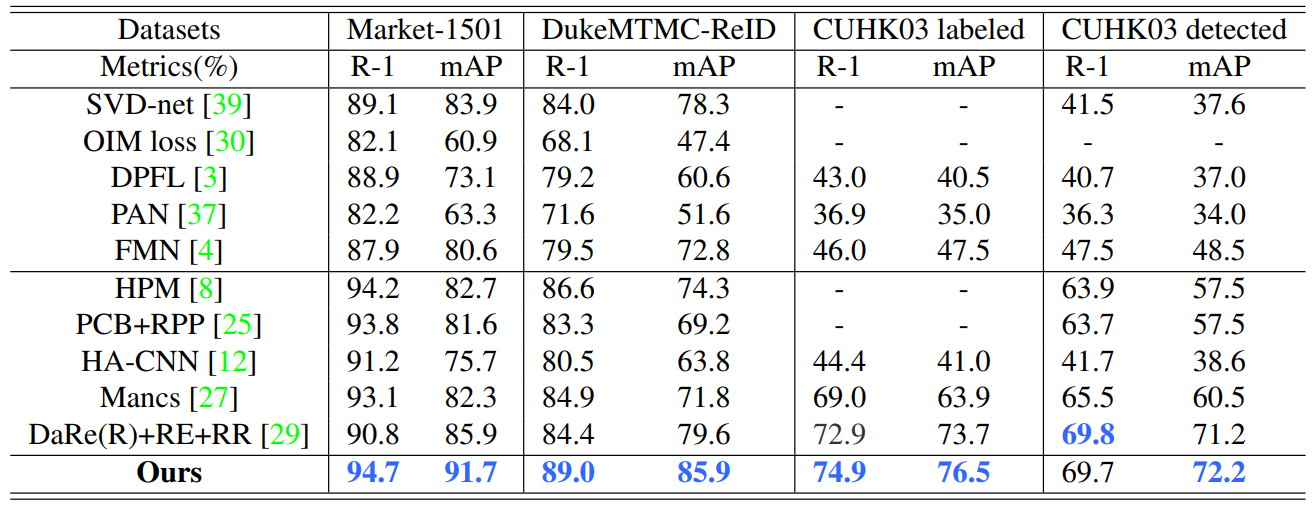
\includegraphics[width=0.8\textwidth]{Chapters/Fig/person-re-id-performance.png}
    \caption{Results of Parameter-free Spatial Attention Network for Person Re-identification in large-scale person re-identification dataset,
    \textbf{Ours} denoted for \cite{SA}}
    \label{fig:sa_results}
\end{figure}
Combining the idea of using a better architecture in person re-identification problem to extract feature vector and the state-of-the-art performance of
\cite{SA} in person re-identification problem, we would like to propose an architecture with the baseline based on \cite{Wojke2017simple} integrating with \cite{SA}
in the \textit{Appearance information measurement} state or DeepSORT with Parameter-free Spatial Attention for extracting appearance features (SADeepSORT). The workflow diagram of SADeepSORT is shown
in fig.\ref{fig:sa_matching}. Result of this combination is compared with the \cite{Wojke2017simple} in the next chapter. 
\begin{figure}[h!]
    \centering
    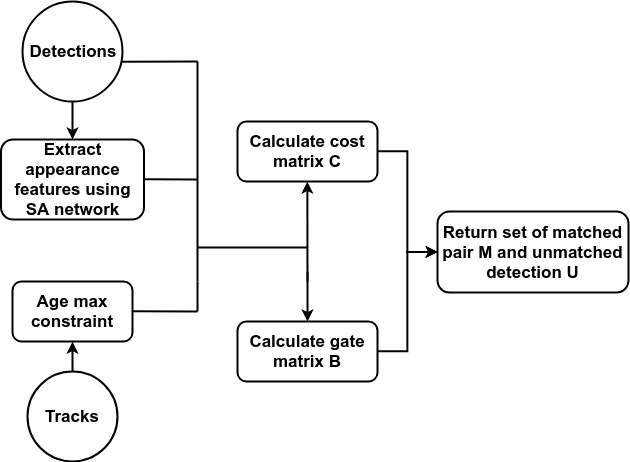
\includegraphics[width=0.8\textwidth]{Chapters/Fig/Thesis_diagram-SA_Matching_Cascade.png}
    \caption{Spatial Network in Matching Cascade of DeepSORT framework}
    \label{fig:sa_matching}
\end{figure}

\pagebreak
\section{DeepSORT with YOLOv3 detector}

\begin{figure}[h!]
    \centering
    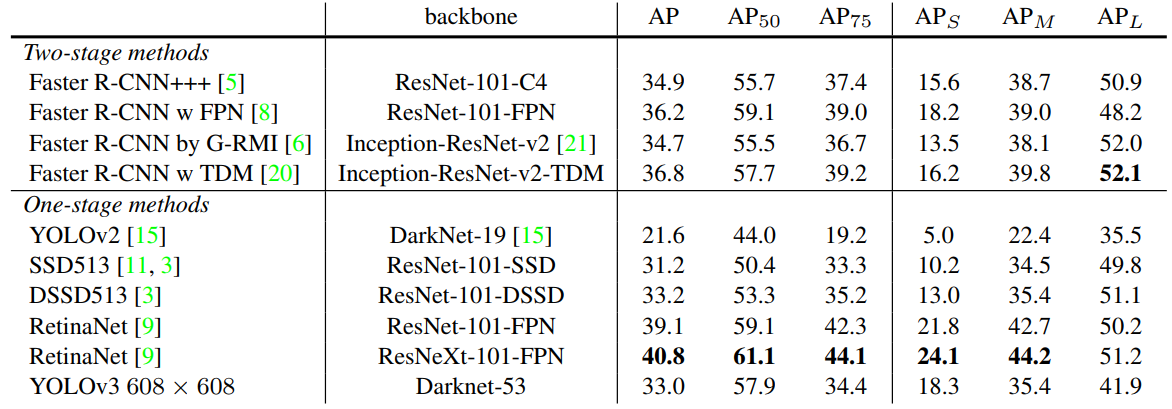
\includegraphics[width=0.7\textwidth]{Chapters/Fig/yolov3_acc_com.png}
    \caption{Accuracy of objects detection algorithms on COCO dataset}
    \label{fig:yolov3_acc_com}
\end{figure}
Fig.\ref{fig:yolov3_acc_com} is showing the result of detection algorithms on COCO dataset,
\cite{yolov3} argues that YOLOv3 is much better than SSD variants and comparable to state-of-the-art
models on the $\text{AP}_{50}$ metric while the computational time is much faster.\par
For the online tracking problem, time constraint is very important, moreover, the quality of the detector makes a proportional effect to the performance of the tracking framework.\par
For all the reasons, we would like to propose DeepSORT with YOLOv3 detector (YOLOv3-DeepSORT) frameworks, the baseline of which now is shown in the fig.\ref{fig:yolo_deepsort} 
\begin{figure}[h!]
    \centering
    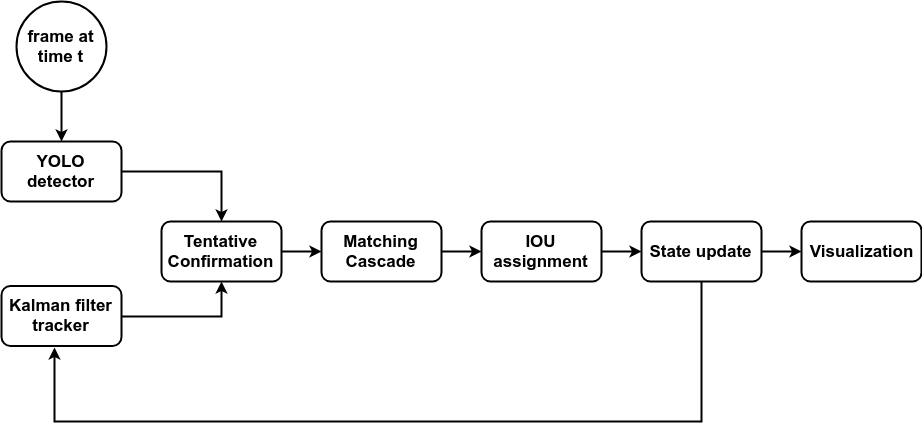
\includegraphics[width=0.8\textwidth]{Chapters/Fig/Thesis_diagram-yolo_deepsort.png}
    \caption{YOLO-DeepSORT's workflow}
    \label{fig:yolo_deepsort}
\end{figure}
